% Created 2024-12-09 pon 19:44
% Intended LaTeX compiler: pdflatex
\documentclass[11pt]{article}
\usepackage[utf8]{inputenc}
\usepackage[T1]{fontenc}
\usepackage{graphicx}
\usepackage{longtable}
\usepackage{wrapfig}
\usepackage{rotating}
\usepackage[normalem]{ulem}
\usepackage{amsmath}
\usepackage{amssymb}
\usepackage{capt-of}
\usepackage{hyperref}
\usepackage[a4paper, margin=1.2in]{geometry}
\hypersetup{colorlinks=true,linkcolor=black}

\newcommand{\SubItem}[1]{
    {\setlength\itemindent{15pt} \item[•] #1}
}

\author{Piotr Jabłoński (325163) i Paweł Wysocki (325248)}
\date{Grudzień 2024}
\title{Dokumentacja wstepna projektu z UMA}
\hypersetup{
 pdfauthor={Piotr Jabłoński (325163) i Paweł Wysocki (325248)},
 pdftitle={Dokumentacja wstepna projektu z UMA},
 pdfkeywords={},
 pdfsubject={},
 pdflang={Polish}}
\begin{document}

\maketitle
\tableofcontents

\pagebreak
\section{Temat projektu}
\label{sec:org004bb5c}
Celem naszego projektu jest implementacja algorytmu konstruującego drzewo klasyfikujące, w którym test dla danego węzła jest wybierany za pomocą ruletki, tj. każdy test ma szansę na wybór proporcjonalną do swojej jakości.
\section{Opis problemu}
\label{sec:org19cc40d}

\subsection{Drzewo klasyfikacyjne}
\label{sec:orgdbf1c0f}

\subsubsection{Ogólna zasada działania}

Drzewo klasyfikacyjne to relatywnie prosty model uczenia maszynowego. Polega on na konstrukcji drzewa binarnego, gdzie:
\begin{itemize}
\item \textbf{węzeł} - atrybut, na podstawie którego dzielimy klasy na podzbiory (tzw. "test")
\item \textbf{liść} - klasa lub predykcja klasy
\end{itemize}
Drzewo można traktować jako wielką instrukcję "if-else" - żeby dojść do liścia, trzeba przejść przez wiele węzłów warunkowych. Kolejne testy w drzewie są wybierane automatycznie, wg wskaźnika \textbf{zysku informacji} (Information Gain) dla danego atrybutu (w każdym węźle wybieramy atrybut, dla którego jest on największy).\\\\
W podstawowej, nieograniczonej wersji drzewa klasyfikacyjnego, dążymy do momentu, gdy wszystkie dane w liściu należą do jednej klasy. Im lepszy test zostanie wybrany do podziału danych, tym precyzyjniejsze będzie nasze drzewo - oznacza to, że celem jest znalezienie takiego testu, dla którego entropia ("nieczystość") zbioru zmniejszy się najbardziej. Jest to ryzykowne podejście, ponieważ czyni ono drzewo bardzo wrażliwym na dane - niewielka zmiana danych wejściowych może znacznie zmienić konstrukcję całego drzewa. Dodatkowo, entropia jest wyliczana dla danych uczących, więc istnieje duże ryzyko przeuczenia drzewa, szczególnie dla niereprezentatywnych zbiorów danych.

\begin{center}
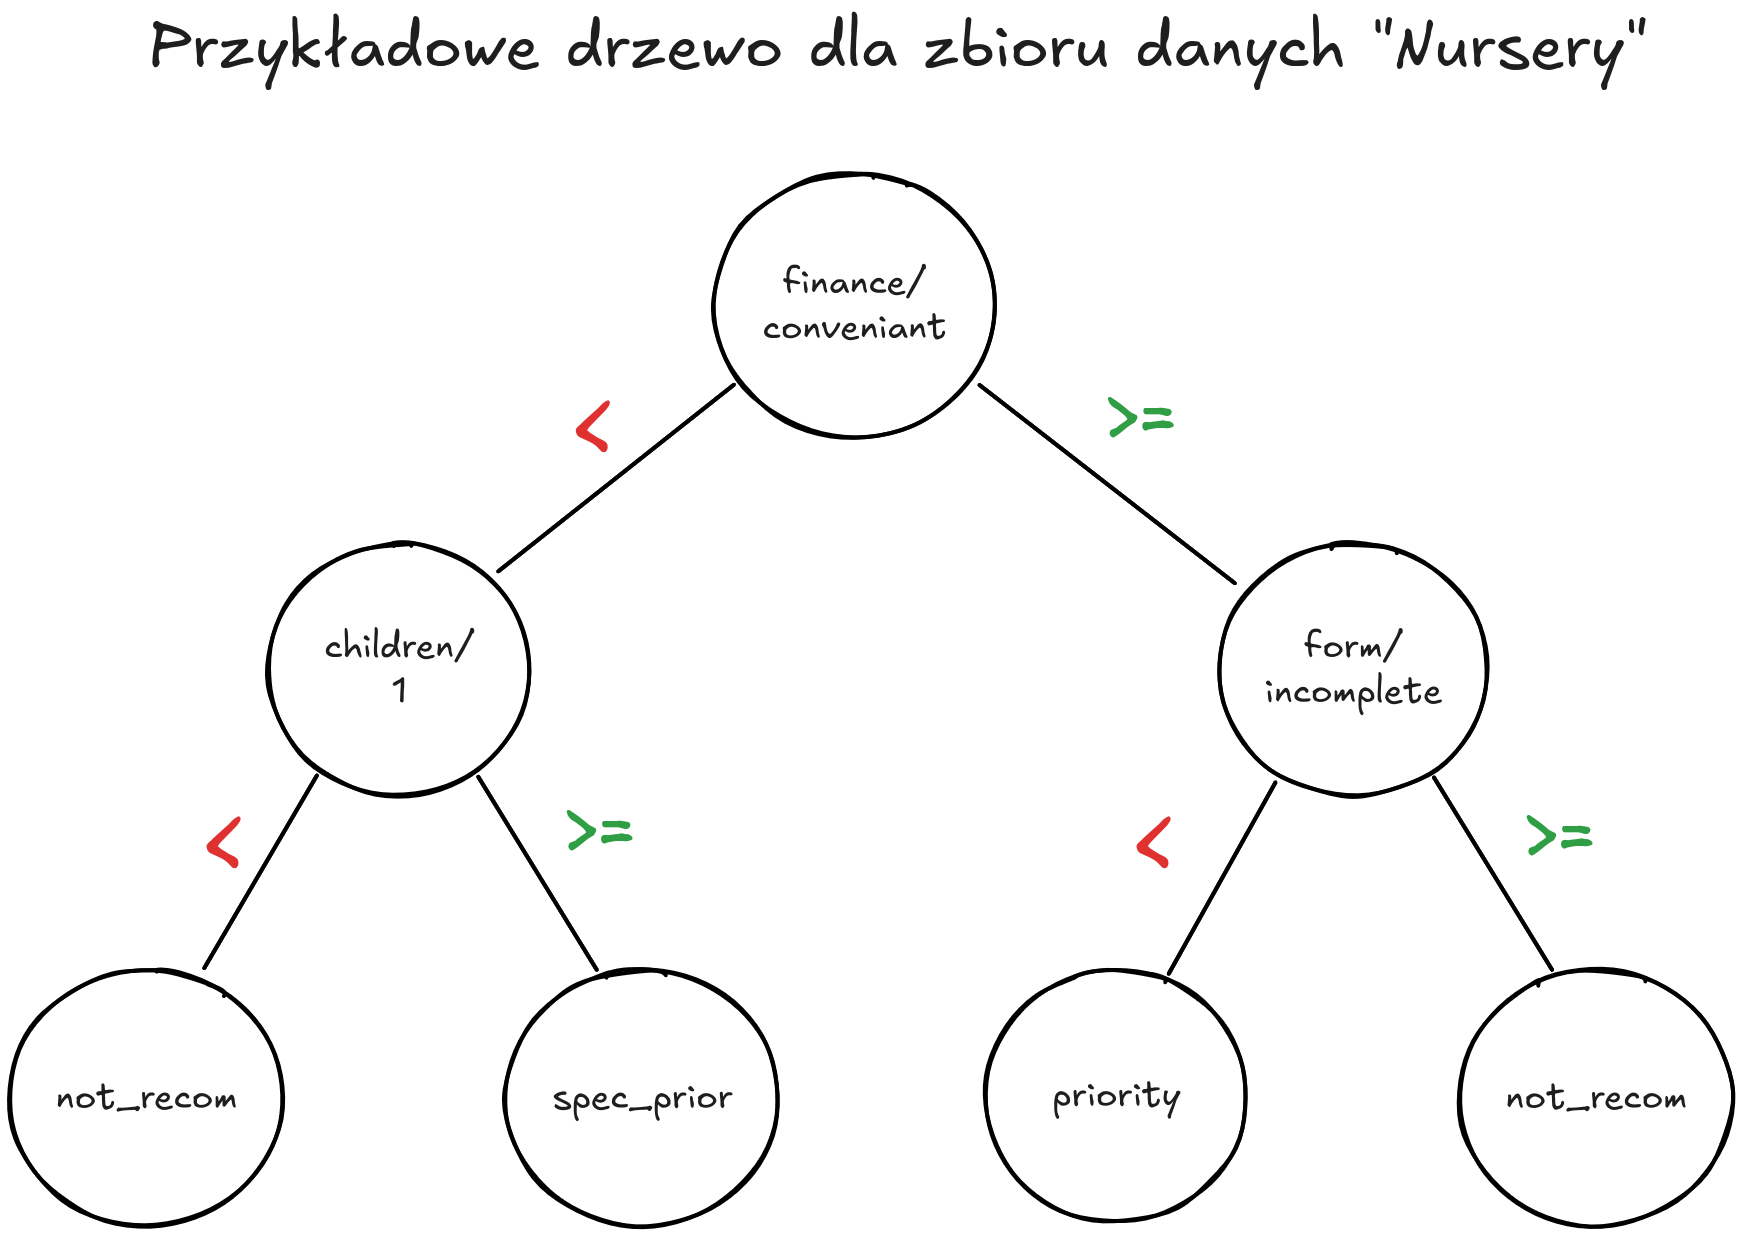
\includegraphics[width=.8\linewidth]{./images/example-nursery-tree.png}
\end{center}

\pagebreak

\subsubsection{Entropia}
\label{ent}\textbf{Entropia} to miara niejednorodności podziału klas. Im większą ma wartość, tym klasy są bardziej wymieszane. Jest obliczana wg wzoru:
$$
E(X) = \sum_{d \in C} -P(c = d)\ \log P(c = d)
$$
gdzie:
\begin{itemize}
\item $X$ - zbiór przykładów w danym węźle
\item $P(c = d)$ - p-stwo wystąpienia klasy $d$ w zbiorze ($\frac{\text{liczba wystąpień klasy $d$ w zbiorze}}{\text{liczba wszystkich elementów w zbiorze}}$)
\end{itemize}
Entropia przyjmuje wartość z przedziału $[0,1]$, dążymy do jej minimalizacji.
\\\\
\label{entwar}\textbf{Entropia warunkowa} określa entropię zbioru po jego podziale danym testem. Oblicza się ją wg wzoru:
$$
E(X|T) = \sum_{t} \frac{|X_t|}{|X|} E(X_t)
$$
gdzie:
\begin{itemize}
\item $t$ - konkretna wartość dla danego testu $T$
\item $|X_t|$ - liczba elementów zbioru, dla których testowany atrybut przyjmuje wartość $t$
\item $|X|$ - liczba wszystkich elementów zbioru $X$
\item $E(X_t)$ - entropia podzbioru $X_t$ zbioru $X$, w którym wszystkie przykłady przyjmują wartość $t$ dla testowanego atrybutu
\end{itemize}
Jest to efektywnie średnia ważona entropii podzbiorów podzielonych testem $T$.

\subsubsection{Kryteria podziału}
Przyjmujemy następujące kryteria podziału w węzłach:
\begin{itemize}
\item\textbf{atrybuty ciągłe}: binarny na podstawie nierówności $a_i \le t$
\item \textbf{atrybuty dyskretne}: binarny na podstawie przynależności do zbioru $a_i \in T$
    \SubItem{wprowadzamy ograniczenie, że zbiór $T$ może zawierać najwyżej połowę wartości atrybutu}
    \SubItem{w teście bierzemy pod uwagę tylko kombinację wartości zawartych w zbiorze $T$, która daje najwyższy przyrost informacji}
\end{itemize}

\newpage
\subsection{Selekcja ruletkowa}
\label{sec:org67ac858}
Zwykłe drzewa decyzyjne są zachłanne, tzn. wybierają ten test, który ma największą jakość. Takie podejście jest proste w realizacji i bardzo efektywne, jednakże czyni drzewo bardzo podatnym na przeuczenie. W naszym przypadku selekcja będzie odbywała się dla każdego testu z zastosowaniem ruletki wg prawdopodobieństwa:
$$
        P(a_i) = \frac{IG(a_i)}{\sum_j^n{IG(a_j)}}
$$
gdzie
\begin{itemize}
\item $P(a_i)$ - prawdopodobieństwo wyboru atrybutu $a_i$
\item $IG(a_i)$ - zysk informacji dla atrybutu $a_i$
\item $\sum_j^n{IG(a_j)}$ - suma zysków informacji dla wszystkich atrybutów możliwych do wyboru w danym węźle
\end{itemize}
Takie podejście sprawia, że prawdopodobieństwo wybrania testu dla atrybutu $a_i$ jest wprost proporcjonalne do zysku informacji, dzięki czemu drzewa powinny mieć mniejszą podatność na przeuczenie. Problem wrażliwości na dane wejściowe również zostanie zredukowany - zmianie będą ulegały prawdopodobieństwa wyboru testu, lecz nie musi to oznaczać zmiany budowy drzewa.
\subsection{Algorytmy}
\label{sec:org4909e92}
Do skonstruowania drzewa klasyfikacyjnego niezbędne są następujące algorytmy:
\begin{itemize}
\item Algorytm budowania drzewa
\item Algorytm wyboru testu z ruletką
\item Algorytm obliczania zysku informacji (\textbf{IG})
\end{itemize}
Poniżej przedstawiamy pseudokody tych algorytmów w języku Pythono-podobnym w celu lepszego zwizualizowania ich działania:
\subsubsection{Algorytm budowania drzewa}
\label{sec:org8d16fe2}
\begin{verbatim}
def build_tree(attrs, data, classes, max_depth) -> DecisionTree:
    if max_depth == 0 or len(attrs) == 0:
        # w przypadku danych niejednorodnych wybieramy najczęstszą klasę
        return most_common(data)
    tree = DecisionTree()

    # przeprowadzamy test z ruletką
    tree.attr, tree.threshold = test(attrs, data, classes)
    new_attr = attrs - tree.attr

    # dzielimy dane na postawie testu
    left_data, right_data = [...]
    tree.left = build_tree(new_attr, left_data, classes, max_depth - 1)
    tree.right = build_tree(new_attr, right_data, classes, max_depth - 1)

    return tree
\end{verbatim}
\subsubsection{Algorytm wyboru testu z ruletką}
\label{sec:orge6811b9}
\begin{verbatim}
def test(attrs, data, classes):
    IGs = []
    for a in attrs:
        IGs.append(IG(a, data, classes))

    # ruletkowy wybór zysku informacji
    total = sum(IGs); running_total = 0; p = randint(0, total)
    probabilities = [ig.gain / total for ig in IGs]
    return numpy.random.choice(IGs, 1, p = probabilities)
\end{verbatim}
\subsubsection{Algorytm obliczania zysku informacji (Information Gain)}
\label{sec:org5372fdc}
\textbf{Information Gain} stosowany jest do mierzenia zmiany entropii dla danego testu. Jest obliczany wg wzoru:
$$
IG(X,T) = E(X) - E(X|T)
$$
gdzie:
\begin{itemize}
\item $E(X)$ - \hyperref[ent]{\underline{entropia}} zbioru $X$
\item $E(X|T)$ - \hyperref[entwar]{\underline{entropia warunkowa}} zbioru $X$ po podziale testem $T$
\end{itemize}
Wskaźnik ten pozwala nam w łatwy sposób określić, jak bardzo dany test wpływa na nasz zbiór danych, więc dążymy do jego maksymalizacji.

\section{Plan eksperymentów}
\label{sec:orgba831bb}
W celu przeprowadzenia odpowiednich testów statystycznych, eksperymenty będą prowadzone na różnych zbiorach danych, a uzyskane wyniki zostaną porównane z klasyfikatorem \href{https://scikit-learn.org/stable/modules/generated/sklearn.tree.DecisionTreeClassifier.html\#decisiontreeclassifier}{DecisionTreeClassifer} z pakietu naukowego \href{https://scikit-learn.org}{scikit-learn}.
\\\\
Macież błędów (tablica pomyłek) posłuży nam do zwizualizowania i zweryfikowania skuteczności klasyfikacji. Będziemy skupiać się na miarach: \textbf{PPV}, \textbf{Recall} i \textbf{F1}.

\section{Zbiory danych}
\label{sec:org34135ba}
Przygotowaliśmy 4 zbiory danych, na których będziemy prowadzić eksperymenty.
\subsection{\href{https://www.kaggle.com/datasets/uciml/red-wine-quality-cortez-et-al-2009/data}{Red Wine Quality}}
\label{sec:orge712876}
Zawiera 11 fizykochemicznych atrybutów win:
\begin{enumerate}
\item Kwasowość stała
\item Kwasowość lotna
\item Kwas cytrynowy
\item Cukier pozostały po fermentacji
\item Chlorki
\item Dwutlenek siarki wolny
\item Dwutlenek siarki całkowity
\item Gęstość
\item pH
\item Siarczany
\item Procent alkoholu
\end{enumerate}
Wszystkie atrybuty są ciągłe, więc zastosowany będzie wyłącznie podział nierównościowy.
\\\\
Zadanie klasyfikacji - \textbf{określenie jakości wina w skali całkowitoliczbowej (1-10)}.
\subsection{\href{https://www.kaggle.com/datasets/taweilo/loan-approval-classification-data}{Loan Approval Classification}}
\label{sec:org43de68f}
Zawiera 9 atrybutów o osobie składającej wniosek o pożyczkę oraz 4 atrybuty o samej pożyczce - łącznie 13 atrybutów, na podstawie których należy sklasyfikować stan wniosku (zaakceptowany bądź odrzucony). Atrybuty:
\begin{enumerate}
\item Wiek
\item Płeć
\item Wykształcenie
\item Dochód roczny
\item Liczba lat doświadczenia zawodowego
\item Stan posiadania domu (wynajem, na własność, hipoteka)
\item Kwota pożyczki
\item Cel pożyczki
\item Oprocentowanie pożyczki
\item Wysokość wypożyczenia w relacji do dochodu rocznego (\%)
\item Zdolność kredytowa
\item Długość historii kredytowej w latach
\item Indykator wcześniejszych niespłaconych wypożyczeń
\end{enumerate}
W tym zbiorze danych występują atrybuty zarówno ciągłe, jak i dyskretne, w związku z czym zostaną wykorzystane oba typy podziałów.
\\\\
Zadanie klasyfikacji - \textbf{akceptacja wniosku o pożyczkę (prawda/fałsz)}.

\subsection{\href{https://www.kaggle.com/datasets/nimapourmoradi/nursery}{Nursery}}
\label{sec:org0f4e062}
Zawiera 8 atrybutów dotyczących rodziny:
\begin{enumerate}
\item Zawód rodziców
\item Jakość zapewnionej opieki nad dzieckiem
\item Struktura rodziny (kompletna, rozbita, itp.)
\item Liczba dzieci
\item Warunki zamieszkania
\item Sytuacja finansowa
\item Sytuacja społeczna
\item Sytuacja zdrowotna
\end{enumerate}
W tym zbiorze występują atrybuty dyskretne, jednakże zostaną zastosowane oba typy podziałów, ponieważ liczbę dzieci da się podzielić nierównościowo.
\\\\
Zadanie klasyfikacji - \textbf{ocena aplikacji do przedszkola (wieloklasowa)}.

\subsection{\href{https://www.kaggle.com/datasets/valakhorasani/mobile-device-usage-and-user-behavior-dataset}{Mobile Device Usage and User Behavior}}
Zawiera 10 atrybutów (korzystamy z 9), które opisują parametry urządzeń mobilnych oraz aktywności użytkowników:
\label{sec:org2f897e3}
\begin{enumerate}
\item Id użytkownika - nieużywane, bo nieistotne
\item Model urządzenia
\item System operacyjny
\item Czas używania aplikacji
\item SOT (Screen On Time)
\item Codzienne zużycie baterii (mAh)
\item Liczba zainstalowanych aplikacji
\item Codzienne zużycie danych (MB)
\item Wiek
\item Płeć (M/K)
\end{enumerate}
W tym zbiorze występują atrybuty ciągłe i dyskretne, więc zostaną zastosowane oba typy podziałów.
\\\\
Zadanie klasyfikacji - \textbf{ocena zachowania użytkownika (od lekkiego do ekstremalnego użycia w skali całkowitoliczbowej 1-5)}.

\end{document}